\section{Theoretical Background}
\label{sec: theory}

\subsection{Convolutional Neural Networks}
\label{subsec: cnn}

CNNs are a type of deep learning architecture inspired by the visual cortex of animals. \cite{Yamashita2018CNN, hubel1968receptive}. They are designed to efficiently capture spatial and temporal dependencies in data through the use of learnable filters and hierarchical feature representations. \cite{Yamashita2018CNN}. Through the use of convolutional layers instead of fully connected layers, the architecture is able to preserve the spatial structure of the input data, making it particularly well-suited for image and video data. This approach not only simplifies pattern detection but also implies a reduction in the number of parameters, which minimizes the necessary computational resources.

Application of CNNs in climate science has yielded several notable contributions, including the reconstruction of the El Nino event of 1877 by Kadow et al. despite extremely limited data availability. \cite{kadow2020}

In the context of this work, an architecture introduced by (\cite{ronneberger2015}) is used, which consists of an encoder and a decoder part as seen in \autoref{fig: u_net}. Due to its shape, it is called U-Net. The encoder part consists of convolutional layers and pooling layers, while the decoder part consists of upscaling layers and in this case, skip connections as proposed by \cite{liu2018inpaining}.

\subsubsection*{Convolutional Layer}
\begin{figure}[H]
    \centering
    \animategraphics[loop,autoplay,width=400pt]{1}{resources/images/convolution_gif/convolution_kernel-}{0}{15}
    \caption{How a convolution operation works. Source: Datahacker.rs. Edge detection. https://datahacker.rs/edge-detection/, 2021.
    Accessed: 2024-05-19.}
    \label{fig: convolution_operation}
\end{figure}

The convolutional layer is the driver for feature mapping in a CNN. It applies a convolution operation shown in \autoref{fig: convolution_operation} to the input data. The operation is done element by element while sliding a filter (also called kernel) over the input data such that situations, where the filter overflows the input data ranges, are avoided or taken care of. On each step, the Frobenius Product between the kernel and the submatrix given by the current position and the kernel dimension is calculated and noted in the output matrix. The parameters in the kernel matrix are chosen in such a way that the Frobenius Product is maximized when the kernel is over a feature that the kernel is supposed to detect. In \autoref{fig: convolution_operation} the kernel for example is a vertical edge detector, meaning it will output a high amount (positive or negative) when the horizontal gradient in the input data submatrix has a high absolute value. This result is rather trivial, as a positive horizontal gradient as seen in the upper-left 3x3 submatrix of the example leads to a right column that when negatively weighted, overweights the positive-weighted left column and thus the output for the upper-left 3x3 submatrix is negative. Conversely, a Fresenius product of the upper-right 3x3 submatrix with the kernel returns a positive value, hinting at a negative horizontal gradient in the input data. The result of such a convolution can be observed in \autoref{fig: edge_detection}.

In the context of weather data, the convolutional layer can be used to detect any weather patterns not just edges and the kernel itself can be learned by the network.

\begin{figure}
    \centering
    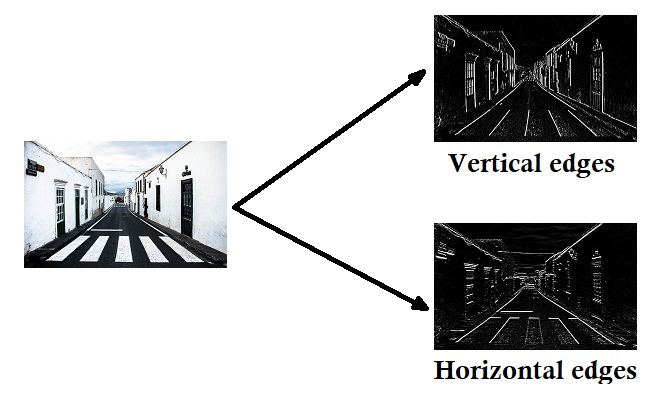
\includegraphics[width=250px]{resources/images/edge_detection.jpeg}
    \caption{Example of edge detection with a convolutional kernel. Source: Datahacker.rs. Edge detection. https://datahacker.rs/edge-detection/, 2021.
    Accessed: 2024-05-19.}
    \label{fig: edge_detection}
\end{figure}

\subsubsection*{Activation Function}

To map the output of the convolutional layer to a meaningful space, and to avoid negative values, an activation function is applied. This introduces non-linearity into the network. The simplest activation function is the ReLU function, which returns the input if it is positive and zero otherwise. It is defined as $f(x) = max(0, x)$. The ReLu function is the activation function used in this work after each convolutional operation.

\begin{figure}[H]
    \begin{subfigure}{1\textwidth}
        \centering
        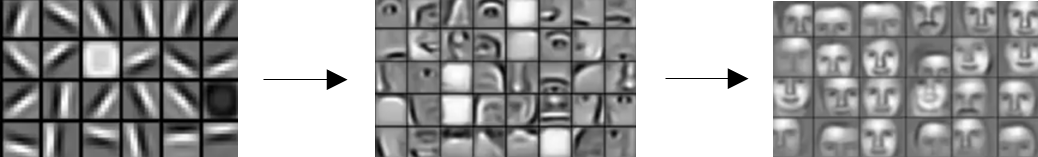
\includegraphics[width=0.9\textwidth]{resources/images/abstraction.png}
        \caption{Low-level features are combined into high-level features.}
        \label{fig: abstraction}
    \end{subfigure}
    \begin{subfigure}{\textwidth}
        \centering
        \vspace{0.5cm}
        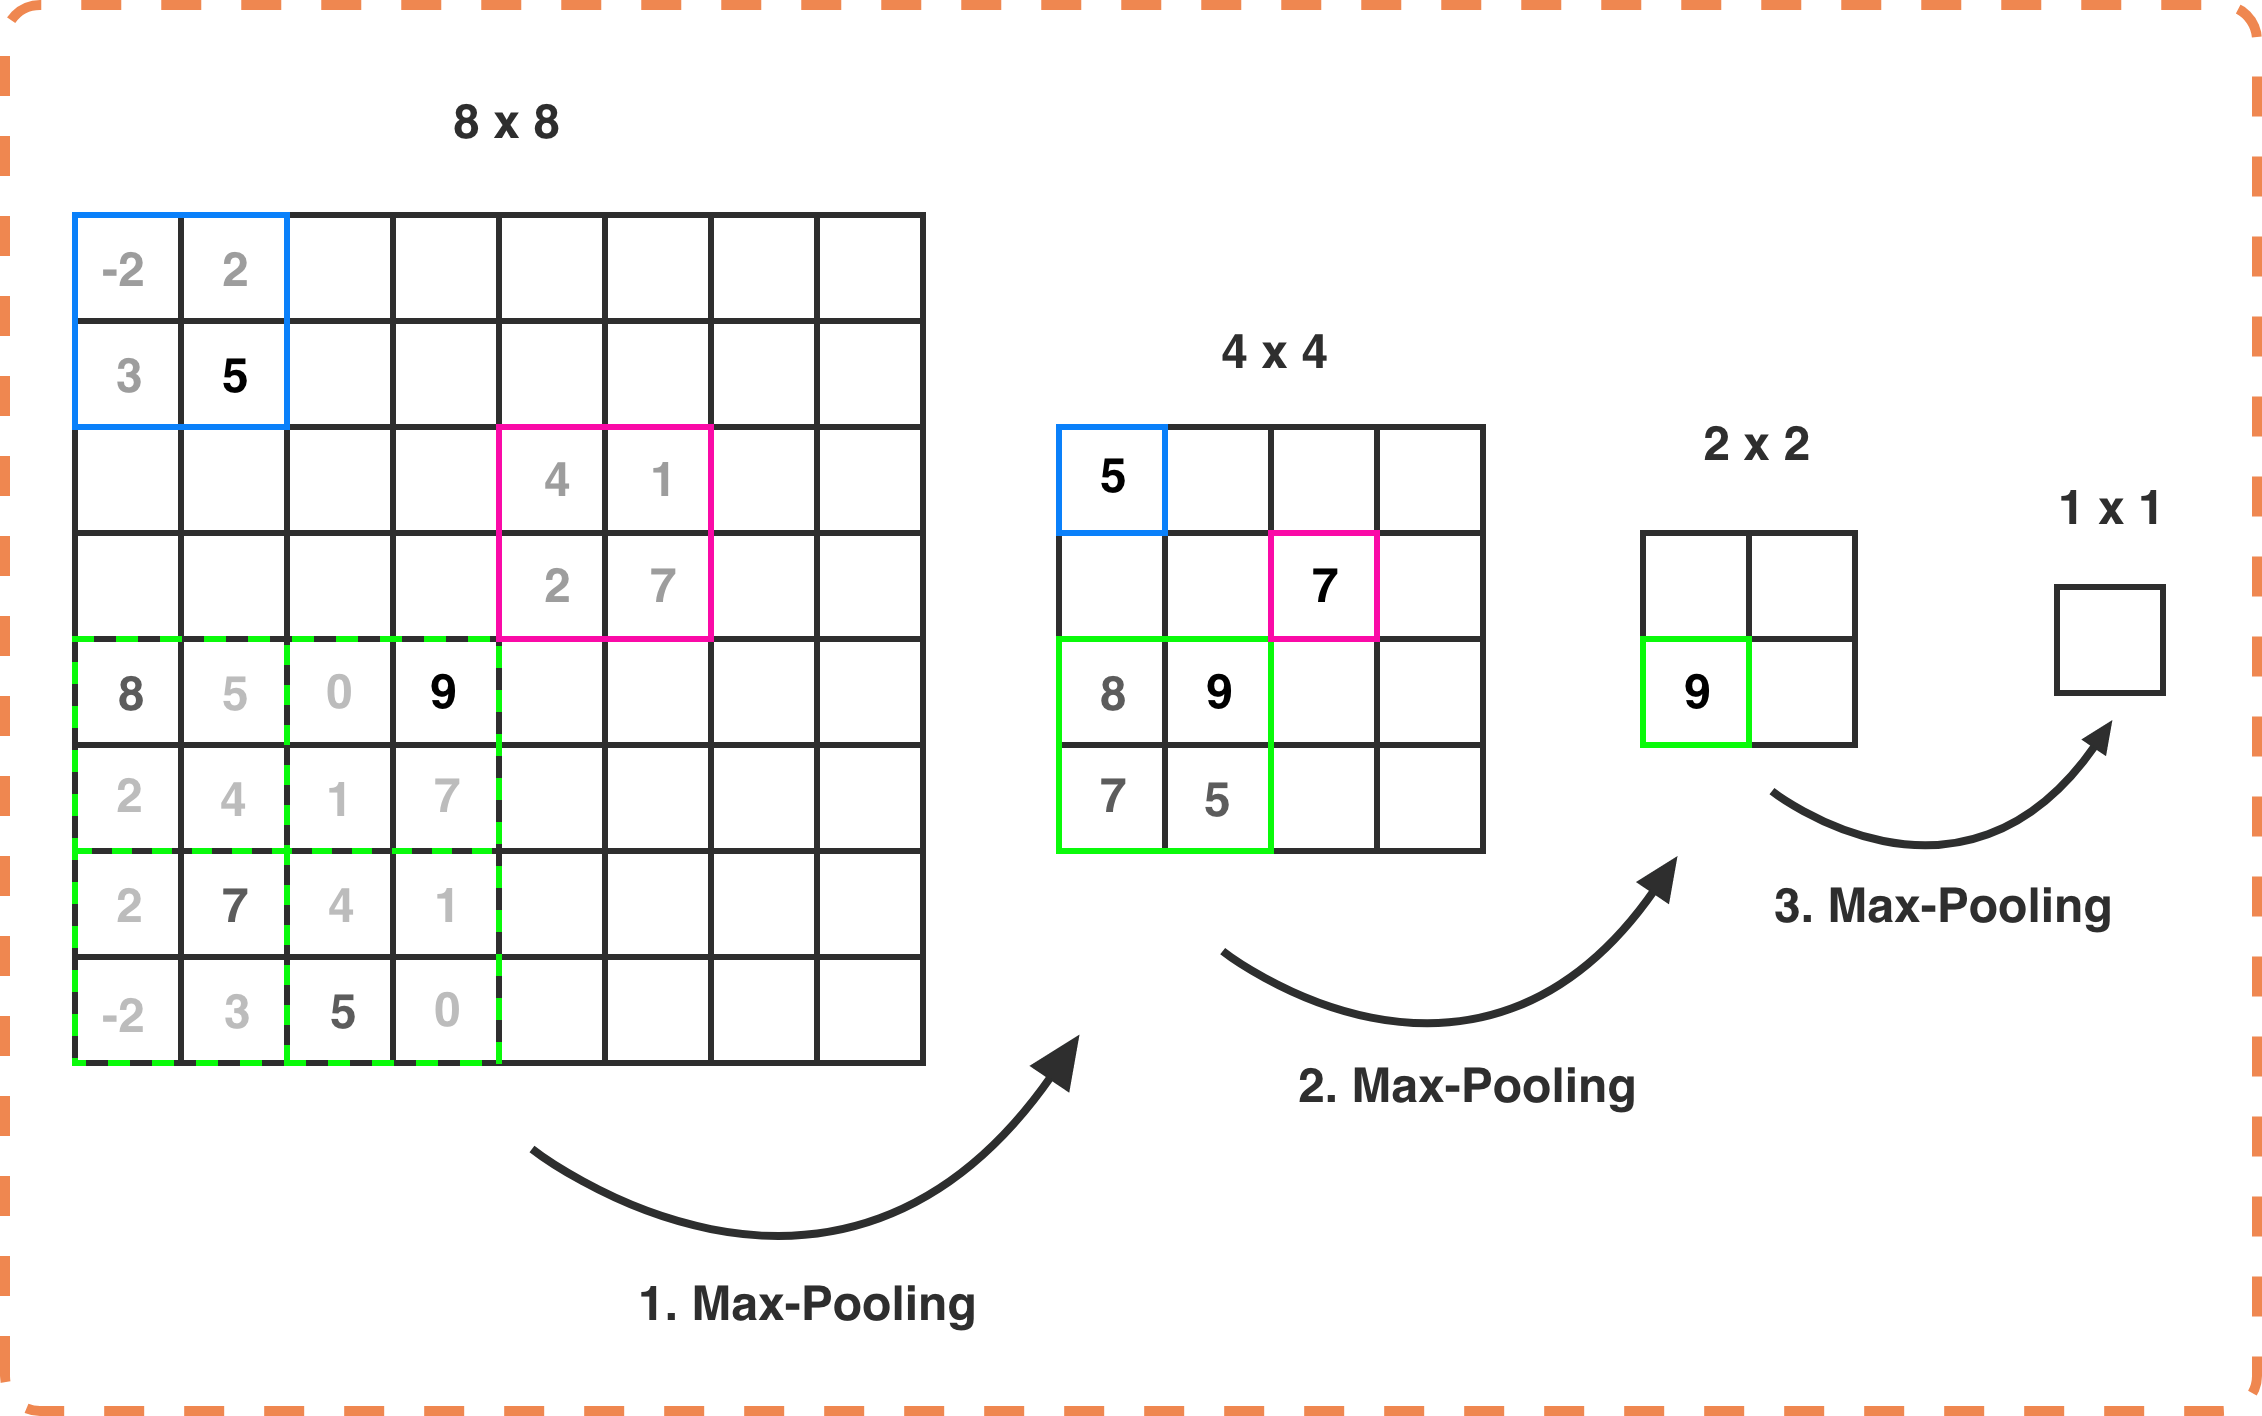
\includegraphics[width=0.7\textwidth]{resources/images/max_pooling.png}
        \caption{Illustration of 3 max pooling operations}
        \label{fig: max_pooling}
    \end{subfigure}
    \begin{subfigure}{\textwidth}
        \centering
        \vspace{0.5cm}
        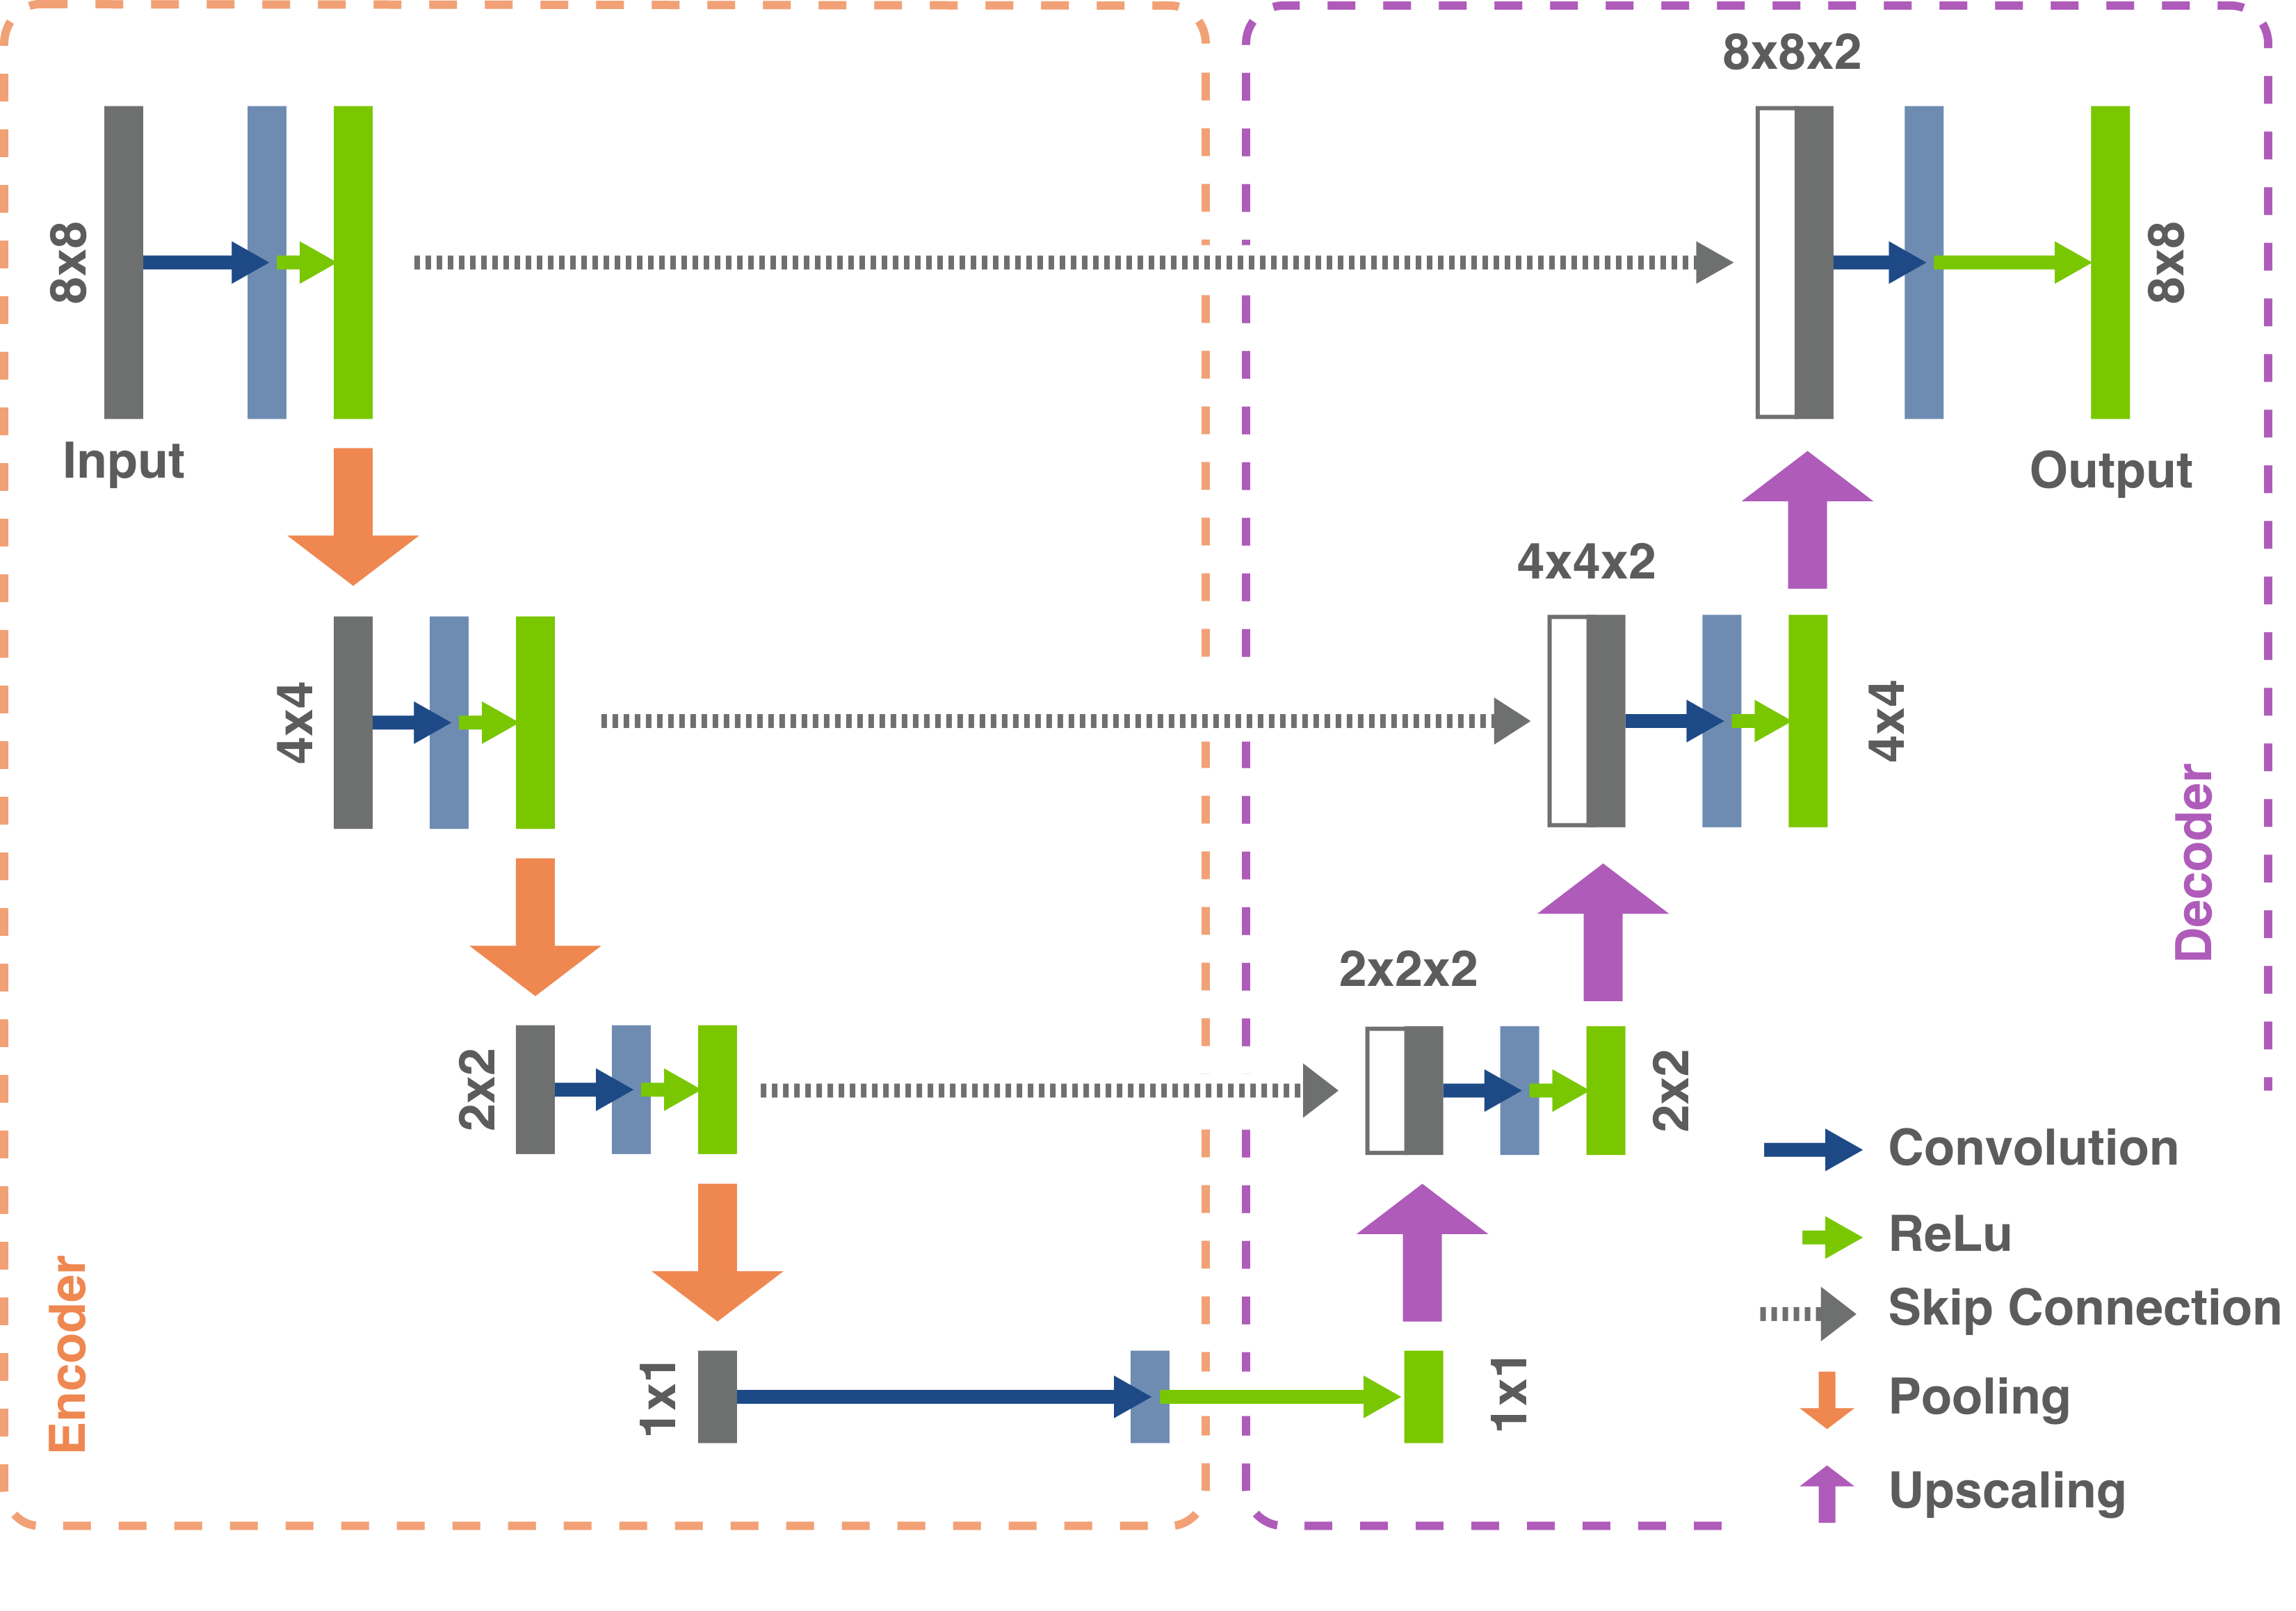
\includegraphics[width=0.9\textwidth]{resources/images/u_net.png}
        \caption{Encoder Decoder Architecture in the U-Net.}
        \label{fig: u_net}
    \end{subfigure}
\end{figure}

\subsubsection*{Pooling Layer}

The exact position of a low-level feature in the input data is not so important when it comes to detecting high-level features,
it is more important to recognize if a feature is present at all in area of the input data or not.
Thus scaling down the resolution of the matrix by combining every 2x2 submatrix into one value can be beneficial.
A possible way to aggregate them is by taking the maximum value of the submatrix, which will work for the mentioned purpose of detecting if a feature is present in the area of the submatrix or not. In \autoref{fig: convolution_operation} the convolution operation itself also reduces the shape of the input data, which is because close to the borders of the input data the kernel can not be applied entirely, but in this work it is avoided by padding the input data. For the 8x8 grid cells of the ERA5 data, that is used as input in the laid out approach (see \autoref{subsec: data_preprocessing}), the architecture of the CNN could include a maximum of 3 pooling layers, reducing the input data to a 1x1 matrix as seen in \autoref{fig: max_pooling}. \autoref{fig: max_pooling} just illustrates the downsampling of the data, in the actual architecture, pooling layers always come together with convolutional layers and are never applied directly after each other as seen in the encoder part of \autoref{fig: encoder_architecture}.
In this work, the pooling is integrated into the convolution operation by using a step size of 2 when sliding the kernel over the input data, reducing the shape of the data by half in each dimension.

\subsubsection*{Decoder}

In the decoding phase of the U-Net architecture, the original data shape is reinstated by upscaling the encoded layers using detected features. Nearest-neighbor interpolation is employed for this purpose, wherein values in the matrix are replicated as required.
As the decoder progressively restores the shape, it incorporates so-called skip connections with the encoder at each level. Skip connections entail copying the outputs of each encoding layer directly into the decoding process.
This mechanism aids the network in retaining the contextual information of the input data, which proves particularly crucial in spatial infilling tasks, where the reconstruction must align with the available surrounding data \cite{liu2018inpaining}.
To integrate the doubled data from skip connections with the upscaling layers, a convolution operation is applied once more (see Figure \ref{fig: u_net}), with the step size configured to halve the size.
This combined architectural approach ensures that for any input data, the model generates a prediction of the same shape as the input, with the predicted values representing the missing data.
The specific values are determined by the parameters employed in the convolution kernels.

\subsubsection*{Supervised Learning}

With the correct convolution kernels found, the prediction should ideally be the same as the target data.
The training process is devised to find the best kernel parameters, which are called weights in this context.
To minimize any differences between ground through and prediction, the differences first need to be quantified in a loss function.
As the model calculates the prediction hour by hour, we only need to compare the prediction to the measured temperature at the weather station at the same hour.
However, as the prediction is a matrix and the target is a scalar, the absolute differences between the measured temperature and the prediction at each of the 64 data points in the output are added up. 

Then the partial gradient of the loss function concerning each weight in the network is calculated.
This involves recursively applying the chain rule of calculus, a process known as backpropagation. The weights are then adjusted in the opposite direction of the gradient to minimize the loss function.
The magnitude of these adjustments is governed by the learning rate, a pivotal hyperparameter in the training process. 

\subsection{Atmospheric Reanalysis}
 
Combining past weather observations with numerical model-based weather predictions (NWP)
is a data assimilation technique called atmospheric reanalysis, particularly when applied over a long period with a consistent data assimilation system \cite{Poli2016ERA20C, ECMWF2020dataassimilation}. The numerical models have degrees of freedom, allowing for adjustments of parameters, which are chosen in such a way that the model output matches the actual measurements wherever they are available in space and time, may it be from a weather station or a satellite.

An institution providing such reanalyses is the European Centre for Medium-Range Weather Forecasts (ECMWF), and over the years, they have produced several reanalyses, with the most recent one being ERA5 \cite{Hersbach2020ERA5quality}.

Several organizations besides ECMWF produce global atmospheric reanalyses. To name a few leading: MERRA-2 from NASA's Global Modeling and Assimilation Office (GMAO) \cite{Gelaro2017}, JRA-55 from the Japan Meteorological Agency (JMA) \cite{Kobayashi2015}, and CFSR (version 2) from the National Centers for Environmental Prediction (NCEP) \cite{Saha2014}.

ECMWF began its reanalysis efforts with the FGGE project in 1979, followed by ERA-15 in the mid-1990s, ERA-40 in the early 2000s, ERA-Interim in 2008, and the most recent ERA5 reanalysis in 2017 \cite{Hersbach2020ERA5quality}. ERA5, the fifth generation reanalysis from ECMWF, surpasses ERA-Interim in accuracy and completeness \cite{Hersbach2020ERA5quality}, which was previously considered the most accurate global reanalysis product \cite{Beck2019interimWasBest}. This makes ERA5 the optimal choice for input data in this work. ERA5's improved accuracy over ERA-Interim is particularly notable in East Africa, where weather stations are sparse and the 3D-printed weather stations aim to make a significant impact \cite{Gleixner2020ERA5africa}. This justifies using ERA5 as a benchmark for comparing the accuracy of the reconstructions produced in this work.

The ERA5 data is available in grid cells of 0.25° x 0.25°, approximately 28 km x 28 km at the equator, and involves four-dimensional data assimilation, considering latitude, longitude, time, and multiple pressure levels in the atmosphere. The technique used for ERA5 is known as 4D-Var \cite{era5}. Although ERA5 offers numerous variables, this work utilizes only the 2-meter temperature as input for the neural network, corresponding to the measurements targeted by the 3D-printed weather stations. However, for similar or extended approaches, other variables such as wind components and solar radiation could also be considered.